% Options for packages loaded elsewhere
\PassOptionsToPackage{unicode}{hyperref}
\PassOptionsToPackage{hyphens}{url}
%
\documentclass[
]{article}
\usepackage{amsmath,amssymb}
\usepackage{iftex}
\ifPDFTeX
  \usepackage[T1]{fontenc}
  \usepackage[utf8]{inputenc}
  \usepackage{textcomp} % provide euro and other symbols
\else % if luatex or xetex
  \usepackage{unicode-math} % this also loads fontspec
  \defaultfontfeatures{Scale=MatchLowercase}
  \defaultfontfeatures[\rmfamily]{Ligatures=TeX,Scale=1}
\fi
\usepackage{lmodern}
\ifPDFTeX\else
  % xetex/luatex font selection
\fi
% Use upquote if available, for straight quotes in verbatim environments
\IfFileExists{upquote.sty}{\usepackage{upquote}}{}
\IfFileExists{microtype.sty}{% use microtype if available
  \usepackage[]{microtype}
  \UseMicrotypeSet[protrusion]{basicmath} % disable protrusion for tt fonts
}{}
\makeatletter
\@ifundefined{KOMAClassName}{% if non-KOMA class
  \IfFileExists{parskip.sty}{%
    \usepackage{parskip}
  }{% else
    \setlength{\parindent}{0pt}
    \setlength{\parskip}{6pt plus 2pt minus 1pt}}
}{% if KOMA class
  \KOMAoptions{parskip=half}}
\makeatother
\usepackage{xcolor}
\usepackage[margin=1in]{geometry}
\usepackage{color}
\usepackage{fancyvrb}
\newcommand{\VerbBar}{|}
\newcommand{\VERB}{\Verb[commandchars=\\\{\}]}
\DefineVerbatimEnvironment{Highlighting}{Verbatim}{commandchars=\\\{\}}
% Add ',fontsize=\small' for more characters per line
\usepackage{framed}
\definecolor{shadecolor}{RGB}{248,248,248}
\newenvironment{Shaded}{\begin{snugshade}}{\end{snugshade}}
\newcommand{\AlertTok}[1]{\textcolor[rgb]{0.94,0.16,0.16}{#1}}
\newcommand{\AnnotationTok}[1]{\textcolor[rgb]{0.56,0.35,0.01}{\textbf{\textit{#1}}}}
\newcommand{\AttributeTok}[1]{\textcolor[rgb]{0.13,0.29,0.53}{#1}}
\newcommand{\BaseNTok}[1]{\textcolor[rgb]{0.00,0.00,0.81}{#1}}
\newcommand{\BuiltInTok}[1]{#1}
\newcommand{\CharTok}[1]{\textcolor[rgb]{0.31,0.60,0.02}{#1}}
\newcommand{\CommentTok}[1]{\textcolor[rgb]{0.56,0.35,0.01}{\textit{#1}}}
\newcommand{\CommentVarTok}[1]{\textcolor[rgb]{0.56,0.35,0.01}{\textbf{\textit{#1}}}}
\newcommand{\ConstantTok}[1]{\textcolor[rgb]{0.56,0.35,0.01}{#1}}
\newcommand{\ControlFlowTok}[1]{\textcolor[rgb]{0.13,0.29,0.53}{\textbf{#1}}}
\newcommand{\DataTypeTok}[1]{\textcolor[rgb]{0.13,0.29,0.53}{#1}}
\newcommand{\DecValTok}[1]{\textcolor[rgb]{0.00,0.00,0.81}{#1}}
\newcommand{\DocumentationTok}[1]{\textcolor[rgb]{0.56,0.35,0.01}{\textbf{\textit{#1}}}}
\newcommand{\ErrorTok}[1]{\textcolor[rgb]{0.64,0.00,0.00}{\textbf{#1}}}
\newcommand{\ExtensionTok}[1]{#1}
\newcommand{\FloatTok}[1]{\textcolor[rgb]{0.00,0.00,0.81}{#1}}
\newcommand{\FunctionTok}[1]{\textcolor[rgb]{0.13,0.29,0.53}{\textbf{#1}}}
\newcommand{\ImportTok}[1]{#1}
\newcommand{\InformationTok}[1]{\textcolor[rgb]{0.56,0.35,0.01}{\textbf{\textit{#1}}}}
\newcommand{\KeywordTok}[1]{\textcolor[rgb]{0.13,0.29,0.53}{\textbf{#1}}}
\newcommand{\NormalTok}[1]{#1}
\newcommand{\OperatorTok}[1]{\textcolor[rgb]{0.81,0.36,0.00}{\textbf{#1}}}
\newcommand{\OtherTok}[1]{\textcolor[rgb]{0.56,0.35,0.01}{#1}}
\newcommand{\PreprocessorTok}[1]{\textcolor[rgb]{0.56,0.35,0.01}{\textit{#1}}}
\newcommand{\RegionMarkerTok}[1]{#1}
\newcommand{\SpecialCharTok}[1]{\textcolor[rgb]{0.81,0.36,0.00}{\textbf{#1}}}
\newcommand{\SpecialStringTok}[1]{\textcolor[rgb]{0.31,0.60,0.02}{#1}}
\newcommand{\StringTok}[1]{\textcolor[rgb]{0.31,0.60,0.02}{#1}}
\newcommand{\VariableTok}[1]{\textcolor[rgb]{0.00,0.00,0.00}{#1}}
\newcommand{\VerbatimStringTok}[1]{\textcolor[rgb]{0.31,0.60,0.02}{#1}}
\newcommand{\WarningTok}[1]{\textcolor[rgb]{0.56,0.35,0.01}{\textbf{\textit{#1}}}}
\usepackage{graphicx}
\makeatletter
\def\maxwidth{\ifdim\Gin@nat@width>\linewidth\linewidth\else\Gin@nat@width\fi}
\def\maxheight{\ifdim\Gin@nat@height>\textheight\textheight\else\Gin@nat@height\fi}
\makeatother
% Scale images if necessary, so that they will not overflow the page
% margins by default, and it is still possible to overwrite the defaults
% using explicit options in \includegraphics[width, height, ...]{}
\setkeys{Gin}{width=\maxwidth,height=\maxheight,keepaspectratio}
% Set default figure placement to htbp
\makeatletter
\def\fps@figure{htbp}
\makeatother
\setlength{\emergencystretch}{3em} % prevent overfull lines
\providecommand{\tightlist}{%
  \setlength{\itemsep}{0pt}\setlength{\parskip}{0pt}}
\setcounter{secnumdepth}{-\maxdimen} % remove section numbering
\ifLuaTeX
  \usepackage{selnolig}  % disable illegal ligatures
\fi
\usepackage{bookmark}
\IfFileExists{xurl.sty}{\usepackage{xurl}}{} % add URL line breaks if available
\urlstyle{same}
\hypersetup{
  hidelinks,
  pdfcreator={LaTeX via pandoc}}

\author{}
\date{\vspace{-2.5em}}

\begin{document}

\newpage
\begin{titlepage}
\begin{center}

\large
UNIVERSIDADE FEDERAL DE UBERLÂNDIA\\
FACULDADE DE ENGENHARIA ELÉTRICA\\
GRADUAÇÃO EM ENGENHARIA BIOMÉDICA\\[7cm]

\Large
\textbf{Heitor Pereira Nunes Fernandes Cunha}\\[2cm]

\textbf{\large Processamento de Sinais Biomédicos: Módulo 8}\\[10cm]

\large
Uberlândia, MG\\
2025

\end{center}
\end{titlepage}

\newpage
\section*{Questão 1}

\begin{quote}
Questão 1
\end{quote}

Dado a frequência f = 0.3rad/s, calcule os valores de frequência em
ciclos/s, rad/amostra e ciclos/amostra. Assuma o valor de fs = 200 Hz.

\begin{Shaded}
\begin{Highlighting}[]
\CommentTok{\# Definindo os valores}
\NormalTok{omega }\OtherTok{\textless{}{-}} \FloatTok{0.3}     \CommentTok{\# Frequência em rad/s}
\NormalTok{fs }\OtherTok{\textless{}{-}} \DecValTok{200}        \CommentTok{\# Frequência de amostragem em Hz (amostras/s)}

\CommentTok{\# 1) Frequência em ciclos/s (Hz)}
\NormalTok{freq\_ciclos\_s }\OtherTok{\textless{}{-}}\NormalTok{ omega }\SpecialCharTok{/}\NormalTok{ (}\DecValTok{2} \SpecialCharTok{*}\NormalTok{ pi)}

\CommentTok{\# 2) Frequência em rad/amostra}
\NormalTok{freq\_rad\_amostra }\OtherTok{\textless{}{-}}\NormalTok{ omega }\SpecialCharTok{/}\NormalTok{ fs}

\CommentTok{\# 3) Frequência em ciclos/amostra}
\NormalTok{freq\_ciclos\_amostra }\OtherTok{\textless{}{-}}\NormalTok{ freq\_ciclos\_s }\SpecialCharTok{/}\NormalTok{ fs}
\CommentTok{\# ou, equivalentemente:}
\CommentTok{\# freq\_ciclos\_amostra \textless{}{-} freq\_rad\_amostra / (2*pi)}

\CommentTok{\# Exibindo os resultados}
\FunctionTok{cat}\NormalTok{(}\StringTok{"Frequência em ciclos/s (Hz) ="}\NormalTok{, freq\_ciclos\_s, }\StringTok{"ciclos/s}\SpecialCharTok{\textbackslash{}n}\StringTok{"}\NormalTok{)}
\end{Highlighting}
\end{Shaded}

\begin{verbatim}
## Frequência em ciclos/s (Hz) = 0.04774648 ciclos/s
\end{verbatim}

\begin{Shaded}
\begin{Highlighting}[]
\FunctionTok{cat}\NormalTok{(}\StringTok{"Frequência em rad/amostra ="}\NormalTok{, freq\_rad\_amostra, }\StringTok{"rad/amostra}\SpecialCharTok{\textbackslash{}n}\StringTok{"}\NormalTok{)}
\end{Highlighting}
\end{Shaded}

\begin{verbatim}
## Frequência em rad/amostra = 0.0015 rad/amostra
\end{verbatim}

\begin{Shaded}
\begin{Highlighting}[]
\FunctionTok{cat}\NormalTok{(}\StringTok{"Frequência em ciclos/amostr ="}\NormalTok{, freq\_ciclos\_amostra, }\StringTok{"ciclos/amostra}\SpecialCharTok{\textbackslash{}n}\StringTok{"}\NormalTok{)}
\end{Highlighting}
\end{Shaded}

\begin{verbatim}
## Frequência em ciclos/amostr = 0.0002387324 ciclos/amostra
\end{verbatim}

\newpage
\section*{Questão 2}

\begin{quote}
Questão 2
\end{quote}

Gere 5 segundos de um sinal s, que deve ser a soma de dois sinais
senoidais, sendo um oscilando a 60 ciclos/s e o outro a 100 ciclos por
segundo. Adote a frequência de amostragem de 1,2 kHZ. Aplique a equação
recursiva ao sinal se responda às questões abaixo:

y{[}n{]} = 1,8523y{[}n-1{]} - 0.94833y{[}n-2{]} + x{[}n{]} -
1.9021x{[}n-1{]} + x{[}n-2{]}

\begin{Shaded}
\begin{Highlighting}[]
\FunctionTok{library}\NormalTok{(dygraphs)}
\FunctionTok{library}\NormalTok{(tidyverse)}
\end{Highlighting}
\end{Shaded}

\begin{verbatim}
## -- Attaching core tidyverse packages ------------------------ tidyverse 2.0.0 --
## v dplyr     1.1.4     v readr     2.1.5
## v forcats   1.0.0     v stringr   1.5.1
## v ggplot2   3.5.1     v tibble    3.2.1
## v lubridate 1.9.3     v tidyr     1.3.1
## v purrr     1.0.2     
## -- Conflicts ------------------------------------------ tidyverse_conflicts() --
## x dplyr::filter() masks stats::filter()
## x dplyr::lag()    masks stats::lag()
## i Use the conflicted package (<http://conflicted.r-lib.org/>) to force all conflicts to become errors
\end{verbatim}

\begin{Shaded}
\begin{Highlighting}[]
\CommentTok{\# Parâmetros de geração do sinal}
\NormalTok{fs }\OtherTok{\textless{}{-}} \DecValTok{1200}           \CommentTok{\# Frequência de amostragem (Hz)}
\NormalTok{T }\OtherTok{\textless{}{-}} \DecValTok{5}               \CommentTok{\# Duração (s)}
\NormalTok{N }\OtherTok{\textless{}{-}}\NormalTok{ T }\SpecialCharTok{*}\NormalTok{ fs          }\CommentTok{\# Número total de amostras}

\CommentTok{\# Vetor de tempo}
\NormalTok{t }\OtherTok{\textless{}{-}} \FunctionTok{seq}\NormalTok{(}\DecValTok{0}\NormalTok{, }\AttributeTok{by =} \DecValTok{1}\SpecialCharTok{/}\NormalTok{fs, }\AttributeTok{length.out =}\NormalTok{ N)}

\CommentTok{\# 2) Gerando o sinal x[n] = sen(2pi60t) + sen(2pi100t)}

\NormalTok{f1 }\OtherTok{\textless{}{-}} \DecValTok{60}             \CommentTok{\# 60 Hz}
\NormalTok{f2 }\OtherTok{\textless{}{-}} \DecValTok{100}            \CommentTok{\# 100 Hz}

\CommentTok{\# Sinais senoidais}
\NormalTok{x1 }\OtherTok{\textless{}{-}} \FunctionTok{sin}\NormalTok{(}\DecValTok{2}\SpecialCharTok{*}\NormalTok{pi}\SpecialCharTok{*}\NormalTok{f1}\SpecialCharTok{*}\NormalTok{t)}
\NormalTok{x2 }\OtherTok{\textless{}{-}} \FunctionTok{sin}\NormalTok{(}\DecValTok{2}\SpecialCharTok{*}\NormalTok{pi}\SpecialCharTok{*}\NormalTok{f2}\SpecialCharTok{*}\NormalTok{t)}

\CommentTok{\# Sinal total de entrada}
\NormalTok{x }\OtherTok{\textless{}{-}}\NormalTok{ x1 }\SpecialCharTok{+}\NormalTok{ x2}

\CommentTok{\# Aplicando a equação recursiva:}

\CommentTok{\# Para armazenar a saída y:}
\NormalTok{y }\OtherTok{\textless{}{-}} \FunctionTok{numeric}\NormalTok{(N)}

\ControlFlowTok{for}\NormalTok{ (n }\ControlFlowTok{in} \DecValTok{3}\SpecialCharTok{:}\NormalTok{N) \{}
\NormalTok{  y[n] }\OtherTok{\textless{}{-}} \FloatTok{1.8523} \SpecialCharTok{*}\NormalTok{ y[n}\DecValTok{{-}1}\NormalTok{] }\SpecialCharTok{{-}} \FloatTok{0.94833} \SpecialCharTok{*}\NormalTok{ y[n}\DecValTok{{-}2}\NormalTok{] }\SpecialCharTok{+}
\NormalTok{          x[n]     }\SpecialCharTok{{-}} \FloatTok{1.9021} \SpecialCharTok{*}\NormalTok{ x[n}\DecValTok{{-}1}\NormalTok{]   }\SpecialCharTok{+}\NormalTok{ x[n}\DecValTok{{-}2}\NormalTok{]}
\NormalTok{\}}

\CommentTok{\# Visualização ou análise de resultados}

\CommentTok{\# Plot do sinal de entrada}
\FunctionTok{plot}\NormalTok{(t[}\DecValTok{1}\SpecialCharTok{:}\NormalTok{(fs)], x[}\DecValTok{1}\SpecialCharTok{:}\NormalTok{(fs)], }\AttributeTok{type =} \StringTok{"l"}\NormalTok{, }
     \AttributeTok{main =} \StringTok{"Sinal de entrada x[n]"}\NormalTok{,}
     \AttributeTok{xlab =} \StringTok{"Tempo (s)"}\NormalTok{, }\AttributeTok{ylab =} \StringTok{"Amplitude"}\NormalTok{)}
\end{Highlighting}
\end{Shaded}

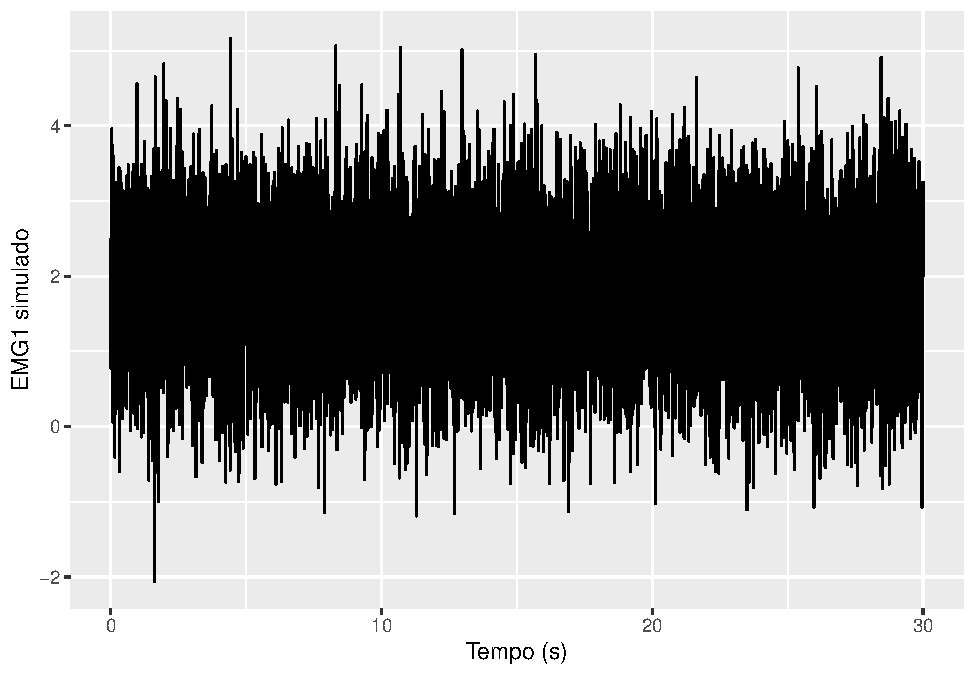
\includegraphics{Modulo8_files/figure-latex/unnamed-chunk-2-1.pdf}

\begin{Shaded}
\begin{Highlighting}[]
\CommentTok{\# Plot do sinal de saída}
\FunctionTok{plot}\NormalTok{(t[}\DecValTok{1}\SpecialCharTok{:}\NormalTok{(fs)], y[}\DecValTok{1}\SpecialCharTok{:}\NormalTok{(fs)], }\AttributeTok{type =} \StringTok{"l"}\NormalTok{, }
     \AttributeTok{main =} \StringTok{"Saída após a equação recursiva"}\NormalTok{,}
     \AttributeTok{xlab =} \StringTok{"Tempo (s)"}\NormalTok{, }\AttributeTok{ylab =} \StringTok{"Amplitude"}\NormalTok{)}
\end{Highlighting}
\end{Shaded}

\includegraphics{Modulo8_files/figure-latex/unnamed-chunk-2-2.pdf}

\begin{quote}
Letra A
\end{quote}

Qual foi o principal efeito de se aplicar a equação de y{[}n{]} sobre o
sinal s?

O principal efeito de aplicar a equação recursiva: y{[}n{]} =
1,8523y{[}n-1{]} - 0.94833y{[}n-2{]} + x{[}n{]} - 1.9021x{[}n-1{]} +
x{[}n-2{]}, sobre o sinal s (soma das senoides de 60 Hz e 100 Hz) é
filtrar essas componentes de frequência de maneira que uma ou ambas
sejam atenuadas ou reforçadas, dependendo de como os polos e zeros do
filtro (definido pelos coeficientes) afetam cada faixa de frequência; em
outras palavras, o filtro modifica a amplitude e a fase das senoides
originais, resultando em um sinal de saída que não é mais a simples soma
das duas ondas, mas sim uma versão alterada por esse sistema de segunda
ordem.

\begin{quote}
Letra B
\end{quote}

Esboce o diagrama de blocos que ilustre o processador descrito por
y{[}n{]}.

\begin{figure}
\centering
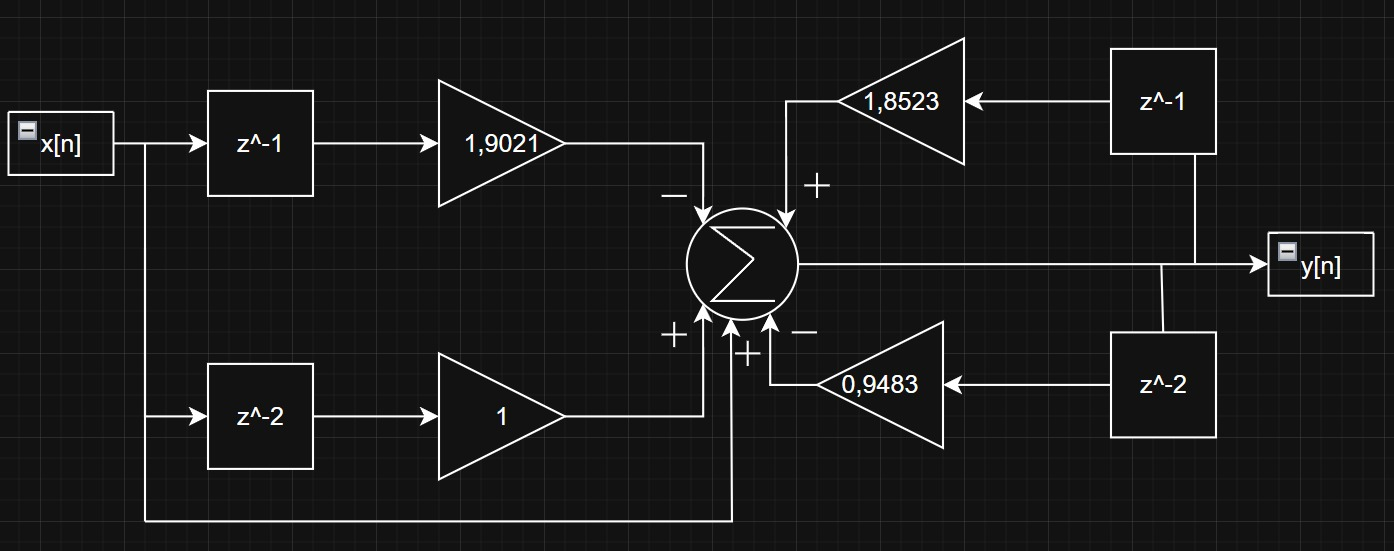
\includegraphics{Diagrama.png}
\caption{Diagrama do sistema}
\end{figure}

\newpage
\section*{Questão 3}

\begin{quote}
Questão 3
\end{quote}

Calcule a resposta ao impulso unitário, h{[}n{]}, para o processador:

y{[}n{]} = y{[}n−1{]} + (1/L)*x{[}n{]} − x{[}n−L{]}.

Para calcular a resposta em frequência, suponhamos que L = 2. Portanto,
temos que aplicar afunção δ{[}n{]} à entrada do sistema, de forma que:

y{[}0{]} = h{[}0{]} = 0 + (1/2)\emph{1 - 0 = 1/2\\
y{[}1{]} = h{[}1{]} = y{[}1-1{]} + (1/2)}x{[}1{]} - x{[}1-2{]} = 1 + 0 +
0 = 1\\
y{[}2{]} = h{[}2{]} = y{[}2-1{]} + (1/2)\emph{x{[}2{]} - x{[}2-2{]} = 0
+ 0 + 1 = 1\\
y{[}3{]} = h{[}3{]} = y{[}3-1{]} + (1/2)}x{[}3{]} - x{[}3-2{]} = 0 + 0 +
0 = 0\\
y{[}4{]} = h{[}4{]} = y{[}4-1{]} + (1/2)*x{[}4{]} - x{[}4-2{]} = 0 + 0 +
0 = 0

Sendo assim, a repsosta ao impulso do problema é: {[}1/2, 1, 1, 0, 0,
\ldots{]}

\newpage
\section*{Questão 4}

\begin{quote}
Questão 4
\end{quote}

Gere 5 segundos de um sinal senoidal amostra a 500 Hz, oscilando a 30
Hz, e adicione ruído gaussiano (com amplitude de no máximo 10\% ao valor
máximo do sinal senoida). Aplique o processador da questão 3 ao sinal
resultante. Qual foi o efeito observado? Plote os gráficos do sinal
origina, corrompido e processado.

\begin{Shaded}
\begin{Highlighting}[]
\CommentTok{\# Carregando pacotes necessários}
\FunctionTok{library}\NormalTok{(tuneR)}
\end{Highlighting}
\end{Shaded}

\begin{verbatim}
## Warning: pacote 'tuneR' foi compilado no R versão 4.4.3
\end{verbatim}

\begin{Shaded}
\begin{Highlighting}[]
\FunctionTok{library}\NormalTok{(dplyr)}
\FunctionTok{library}\NormalTok{(ggplot2)}

\CommentTok{\# Parâmetros do sinal}
\NormalTok{tempo\_final }\OtherTok{\textless{}{-}} \DecValTok{5}
\NormalTok{taxa\_amostragem }\OtherTok{\textless{}{-}} \DecValTok{500}
\NormalTok{frequencia\_sinal }\OtherTok{\textless{}{-}} \DecValTok{30}
\NormalTok{delta\_tempo }\OtherTok{\textless{}{-}} \DecValTok{1} \SpecialCharTok{/}\NormalTok{ taxa\_amostragem}
\NormalTok{vetor\_tempo }\OtherTok{\textless{}{-}} \FunctionTok{seq}\NormalTok{(}\DecValTok{0}\NormalTok{, tempo\_final, }\AttributeTok{by =}\NormalTok{ delta\_tempo)}

\CommentTok{\# Gerando sinal senoidal puro}
\NormalTok{sinal\_puro }\OtherTok{\textless{}{-}} \FunctionTok{sin}\NormalTok{(}\DecValTok{2} \SpecialCharTok{*}\NormalTok{ pi }\SpecialCharTok{*}\NormalTok{ frequencia\_sinal }\SpecialCharTok{*}\NormalTok{ vetor\_tempo)}
\NormalTok{df\_sinal\_puro }\OtherTok{\textless{}{-}} \FunctionTok{data.frame}\NormalTok{(}\AttributeTok{tempo =}\NormalTok{ vetor\_tempo, }\AttributeTok{valor =}\NormalTok{ sinal\_puro, }\AttributeTok{tipo =} \StringTok{"Sinal Original"}\NormalTok{)}

\CommentTok{\# Gerando ruído branco}
\NormalTok{sinal\_ruido }\OtherTok{\textless{}{-}} \FunctionTok{noise}\NormalTok{(}\AttributeTok{kind =} \StringTok{"white"}\NormalTok{, }\AttributeTok{duration =}\NormalTok{ tempo\_final }\SpecialCharTok{+}\NormalTok{ delta\_tempo,}
                     \AttributeTok{samp.rate =}\NormalTok{ taxa\_amostragem, }\AttributeTok{xunit =} \StringTok{"time"}\NormalTok{)}\SpecialCharTok{@}\NormalTok{left}

\CommentTok{\# Sinal corrompido com ruído}
\NormalTok{sinal\_ruidoso }\OtherTok{\textless{}{-}}\NormalTok{ sinal\_puro }\SpecialCharTok{+}\NormalTok{ sinal\_ruido}
\NormalTok{df\_ruidoso }\OtherTok{\textless{}{-}} \FunctionTok{data.frame}\NormalTok{(}\AttributeTok{tempo =}\NormalTok{ vetor\_tempo, }\AttributeTok{valor =}\NormalTok{ sinal\_ruidoso, }\AttributeTok{tipo =} \StringTok{"Sinal Corrompido"}\NormalTok{)}

\CommentTok{\# Preparando estrutura para processamento do sinal}
\NormalTok{df\_processado }\OtherTok{\textless{}{-}}\NormalTok{ df\_sinal\_puro }\SpecialCharTok{\%\textgreater{}\%}
  \FunctionTok{mutate}\NormalTok{(}
    \AttributeTok{xn  =}\NormalTok{ valor,}
    \AttributeTok{xn1 =} \FunctionTok{lag}\NormalTok{(valor, }\DecValTok{1}\NormalTok{) }\SpecialCharTok{*}\NormalTok{ (}\SpecialCharTok{{-}}\FloatTok{1.9021}\NormalTok{),}
    \AttributeTok{xn2 =} \FunctionTok{lag}\NormalTok{(valor, }\DecValTok{2}\NormalTok{)}
\NormalTok{  )}

\CommentTok{\# Inicializando vetor de saída processada}
\NormalTok{saida\_filtrada }\OtherTok{\textless{}{-}} \FunctionTok{rep}\NormalTok{(}\ConstantTok{NA}\NormalTok{, }\FunctionTok{length}\NormalTok{(vetor\_tempo))}
\NormalTok{saida\_filtrada[}\DecValTok{1}\SpecialCharTok{:}\DecValTok{2}\NormalTok{] }\OtherTok{\textless{}{-}} \DecValTok{0}

\CommentTok{\# Aplicando filtro IIR}
\ControlFlowTok{for}\NormalTok{ (i }\ControlFlowTok{in} \DecValTok{3}\SpecialCharTok{:}\FunctionTok{length}\NormalTok{(saida\_filtrada)) \{}
\NormalTok{  entrada\_sum }\OtherTok{\textless{}{-}} \FunctionTok{sum}\NormalTok{(df\_processado}\SpecialCharTok{$}\NormalTok{xn[i],}
\NormalTok{                     df\_processado}\SpecialCharTok{$}\NormalTok{xn1[i],}
\NormalTok{                     df\_processado}\SpecialCharTok{$}\NormalTok{xn2[i], }\AttributeTok{na.rm =} \ConstantTok{TRUE}\NormalTok{)}
  
\NormalTok{  saida\_filtrada[i] }\OtherTok{\textless{}{-}} \FloatTok{1.8523} \SpecialCharTok{*}\NormalTok{ saida\_filtrada[i }\SpecialCharTok{{-}} \DecValTok{1}\NormalTok{] }\SpecialCharTok{{-}}
                       \FloatTok{0.94833} \SpecialCharTok{*}\NormalTok{ saida\_filtrada[i }\SpecialCharTok{{-}} \DecValTok{2}\NormalTok{] }\SpecialCharTok{+}
\NormalTok{                       entrada\_sum}
\NormalTok{\}}

\CommentTok{\# Montando o data frame do sinal processado}
\NormalTok{df\_final }\OtherTok{\textless{}{-}} \FunctionTok{data.frame}\NormalTok{(}\AttributeTok{tempo =}\NormalTok{ vetor\_tempo,}
                       \AttributeTok{valor =}\NormalTok{ saida\_filtrada,}
                       \AttributeTok{tipo =} \StringTok{"Sinal Processado"}\NormalTok{)}

\CommentTok{\# Combinando todos os sinais para visualização}
\NormalTok{df\_completo }\OtherTok{\textless{}{-}} \FunctionTok{bind\_rows}\NormalTok{(}
\NormalTok{  df\_sinal\_puro }\SpecialCharTok{\%\textgreater{}\%} \FunctionTok{rename}\NormalTok{(}\AttributeTok{tempo =}\NormalTok{ tempo, }\AttributeTok{valor =}\NormalTok{ valor) }\SpecialCharTok{\%\textgreater{}\%} \FunctionTok{select}\NormalTok{(tempo, valor, tipo),}
\NormalTok{  df\_ruidoso,}
\NormalTok{  df\_final}
\NormalTok{)}

\CommentTok{\# Garantindo a ordem correta dos painéis}
\NormalTok{df\_completo}\SpecialCharTok{$}\NormalTok{tipo }\OtherTok{\textless{}{-}} \FunctionTok{factor}\NormalTok{(df\_completo}\SpecialCharTok{$}\NormalTok{tipo,}
                           \AttributeTok{levels =} \FunctionTok{c}\NormalTok{(}\StringTok{"Sinal Original"}\NormalTok{, }\StringTok{"Sinal Corrompido"}\NormalTok{, }\StringTok{"Sinal Processado"}\NormalTok{))}

\CommentTok{\# Criando gráfico em painel (facet)}
\NormalTok{painel }\OtherTok{\textless{}{-}} \FunctionTok{ggplot}\NormalTok{(df\_completo, }\FunctionTok{aes}\NormalTok{(}\AttributeTok{x =}\NormalTok{ tempo, }\AttributeTok{y =}\NormalTok{ valor)) }\SpecialCharTok{+}
  \FunctionTok{geom\_line}\NormalTok{(}\AttributeTok{color =} \StringTok{"darkgreen"}\NormalTok{) }\SpecialCharTok{+}
  \FunctionTok{facet\_wrap}\NormalTok{(}\SpecialCharTok{\textasciitilde{}}\NormalTok{ tipo, }\AttributeTok{nrow =} \DecValTok{3}\NormalTok{, }\AttributeTok{scales =} \StringTok{"free\_y"}\NormalTok{) }\SpecialCharTok{+}
  \FunctionTok{labs}\NormalTok{(}\AttributeTok{x =} \StringTok{"Tempo (s)"}\NormalTok{, }\AttributeTok{y =} \StringTok{"Amplitude"}\NormalTok{) }\SpecialCharTok{+}
  \FunctionTok{theme\_minimal}\NormalTok{(}\AttributeTok{base\_size =} \DecValTok{14}\NormalTok{)}

\CommentTok{\# Exibindo gráfico}
\NormalTok{painel}
\end{Highlighting}
\end{Shaded}

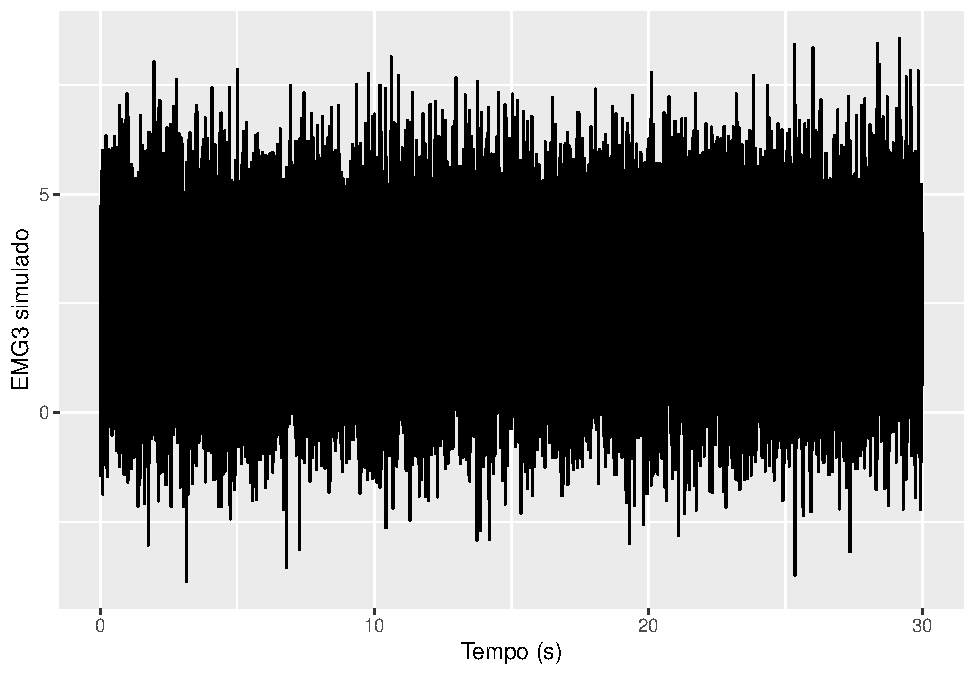
\includegraphics{Modulo8_files/figure-latex/unnamed-chunk-3-1.pdf}
\newpage

\section*{Questão 5}

\begin{quote}
Questão 5
\end{quote}

Calcule a resposta em frequência, H(z) de
y{[}n{]}=0.5{[}x(n)+x{[}n−1{]}{]}. Faça o gráfico da amplitude e fase.
Que tipo de processador é esse?

\begin{Shaded}
\begin{Highlighting}[]
\CommentTok{\# Carregar bibliotecas necessárias}
\FunctionTok{library}\NormalTok{(signal)}
\end{Highlighting}
\end{Shaded}

\begin{verbatim}
## Warning: pacote 'signal' foi compilado no R versão 4.4.3
\end{verbatim}

\begin{verbatim}
## 
## Anexando pacote: 'signal'
\end{verbatim}

\begin{verbatim}
## O seguinte objeto é mascarado por 'package:dplyr':
## 
##     filter
\end{verbatim}

\begin{verbatim}
## Os seguintes objetos são mascarados por 'package:stats':
## 
##     filter, poly
\end{verbatim}

\begin{Shaded}
\begin{Highlighting}[]
\FunctionTok{library}\NormalTok{(REdaS)}
\end{Highlighting}
\end{Shaded}

\begin{verbatim}
## Warning: pacote 'REdaS' foi compilado no R versão 4.4.3
\end{verbatim}

\begin{verbatim}
## Carregando pacotes exigidos: grid
\end{verbatim}

\begin{Shaded}
\begin{Highlighting}[]
\FunctionTok{library}\NormalTok{(ggplot2)}

\NormalTok{numerador }\OtherTok{\textless{}{-}} \FunctionTok{c}\NormalTok{(}\FloatTok{0.5}\NormalTok{, }\FloatTok{0.5}\NormalTok{)}
\NormalTok{denominador }\OtherTok{\textless{}{-}} \FunctionTok{c}\NormalTok{(}\DecValTok{1}\NormalTok{)}
\NormalTok{taxa\_amostragem }\OtherTok{\textless{}{-}} \DecValTok{500}

\CommentTok{\# Calcular a resposta em frequência do filtro}
\NormalTok{resposta\_freq }\OtherTok{\textless{}{-}} \FunctionTok{freqz}\NormalTok{(numerador, denominador, }\AttributeTok{Fs =}\NormalTok{ taxa\_amostragem)}

\CommentTok{\# Obter módulo da resposta em frequência}
\NormalTok{modulo }\OtherTok{\textless{}{-}} \FunctionTok{Mod}\NormalTok{(resposta\_freq}\SpecialCharTok{$}\NormalTok{h)}

\CommentTok{\# Calcular fase em radianos e converter para graus}
\NormalTok{fase\_rad }\OtherTok{\textless{}{-}} \FunctionTok{Arg}\NormalTok{(resposta\_freq}\SpecialCharTok{$}\NormalTok{h)}
\NormalTok{fase\_graus }\OtherTok{\textless{}{-}} \FunctionTok{rad2deg}\NormalTok{(fase\_rad)}

\CommentTok{\# Converter módulo para escala decibéis}
\NormalTok{modulo\_db }\OtherTok{\textless{}{-}} \DecValTok{20} \SpecialCharTok{*} \FunctionTok{log10}\NormalTok{(modulo)}

\CommentTok{\# Criar dataframe com os resultados para visualização}
\NormalTok{dados\_plot }\OtherTok{\textless{}{-}} \FunctionTok{data.frame}\NormalTok{(}
  \AttributeTok{frequencia =}\NormalTok{ resposta\_freq}\SpecialCharTok{$}\NormalTok{f,}
  \AttributeTok{resposta\_complexa =}\NormalTok{ resposta\_freq}\SpecialCharTok{$}\NormalTok{h,}
\NormalTok{  fase\_rad,}
\NormalTok{  fase\_graus,}
\NormalTok{  modulo,}
\NormalTok{  modulo\_db}
\NormalTok{)}

\CommentTok{\# Gráfico do módulo}
\FunctionTok{ggplot}\NormalTok{(dados\_plot, }\FunctionTok{aes}\NormalTok{(}\AttributeTok{x =}\NormalTok{ frequencia, }\AttributeTok{y =}\NormalTok{ modulo)) }\SpecialCharTok{+}
  \FunctionTok{geom\_line}\NormalTok{() }\SpecialCharTok{+}
  \FunctionTok{theme\_classic}\NormalTok{() }\SpecialCharTok{+}
  \FunctionTok{labs}\NormalTok{(}\AttributeTok{title =} \StringTok{"Módulo da Resposta em Frequência"}\NormalTok{, }\AttributeTok{x =} \StringTok{"Frequência (Hz)"}\NormalTok{, }\AttributeTok{y =} \StringTok{"|H(f)|"}\NormalTok{)}
\end{Highlighting}
\end{Shaded}

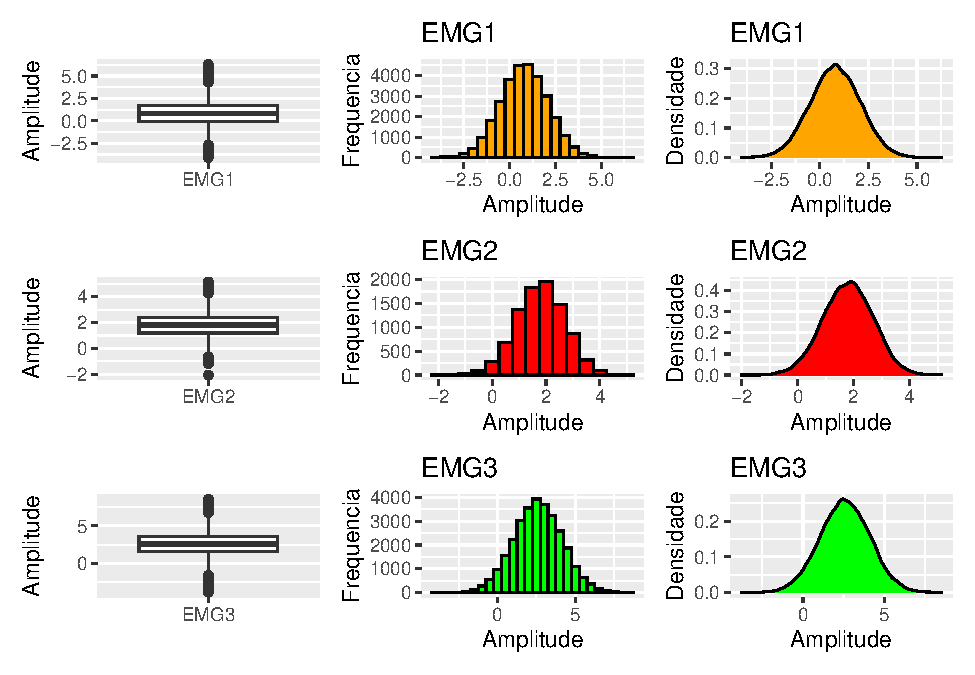
\includegraphics{Modulo8_files/figure-latex/unnamed-chunk-4-1.pdf}

\begin{Shaded}
\begin{Highlighting}[]
\CommentTok{\# Gráfico da fase em graus}
\FunctionTok{ggplot}\NormalTok{(dados\_plot, }\FunctionTok{aes}\NormalTok{(}\AttributeTok{x =}\NormalTok{ frequencia, }\AttributeTok{y =}\NormalTok{ fase\_graus)) }\SpecialCharTok{+}
  \FunctionTok{geom\_line}\NormalTok{() }\SpecialCharTok{+}
  \FunctionTok{theme\_classic}\NormalTok{() }\SpecialCharTok{+}
  \FunctionTok{labs}\NormalTok{(}\AttributeTok{title =} \StringTok{"Fase da Resposta em Frequência"}\NormalTok{, }\AttributeTok{x =} \StringTok{"Frequência (Hz)"}\NormalTok{, }\AttributeTok{y =} \StringTok{"Fase (graus)"}\NormalTok{)}
\end{Highlighting}
\end{Shaded}

\includegraphics{Modulo8_files/figure-latex/unnamed-chunk-4-2.pdf}

\begin{Shaded}
\begin{Highlighting}[]
\CommentTok{\# Gráfico do módulo em decibéis}
\FunctionTok{ggplot}\NormalTok{(dados\_plot, }\FunctionTok{aes}\NormalTok{(}\AttributeTok{x =}\NormalTok{ frequencia, }\AttributeTok{y =}\NormalTok{ modulo\_db)) }\SpecialCharTok{+}
  \FunctionTok{geom\_line}\NormalTok{() }\SpecialCharTok{+}
  \FunctionTok{theme\_classic}\NormalTok{() }\SpecialCharTok{+}
  \FunctionTok{labs}\NormalTok{(}\AttributeTok{title =} \StringTok{"Resposta em Frequência (dB)"}\NormalTok{, }\AttributeTok{x =} \StringTok{"Frequência (Hz)"}\NormalTok{, }\AttributeTok{y =} \StringTok{"Magnitude (dB)"}\NormalTok{)}
\end{Highlighting}
\end{Shaded}

\includegraphics{Modulo8_files/figure-latex/unnamed-chunk-4-3.pdf}
Trata-se de um filtro FIR de 2 coeficientes que efetua a média simples
de duas amostras consecutivas (1/2*{[}x(n)+x(n−1){]}). Em termos de
resposta em frequência, ele se comporta como um filtro passa-baixas,
atenuando as componentes em altas frequências (onde atinge ganho zero em
w = pi) e mantém o ganho máximo de w = 0.

\newpage
\section*{Questão 6}

\begin{quote}
Questão 6
\end{quote}

Simule três bursts de sinais eletromiográficos em um tempo de 10 s. Cada
burst deve ter a duração de 2 segundos. Assuma que o sinal foi amostrado
a 1000 Hz. Promova um ganho de 1.2 vezes nos trecho em que há atividade
eletromiográfica. Filtre o sinal gerado com um fitro passa-baixa, com
frequência de corte de 5 Hz e ordem 3. Faça a comparação entre sinais
filtrados pelos filtros Butterworth e Chebyshev. Plote os gráficos dos
sinais obtidados e as respostas em frequência dos filtros utilizados.
Dicas: (i) para a geração do sinal utilize a função randn. (ii) Para a
filtragem do sinal utilize a função filtfilt.

\begin{Shaded}
\begin{Highlighting}[]
\FunctionTok{library}\NormalTok{(signal)}
\FunctionTok{library}\NormalTok{(dygraphs)}

\NormalTok{taxa\_amostragem }\OtherTok{\textless{}{-}} \DecValTok{1000}
\NormalTok{dt }\OtherTok{\textless{}{-}} \DecValTok{1} \SpecialCharTok{/}\NormalTok{ taxa\_amostragem}
\NormalTok{tempo }\OtherTok{\textless{}{-}} \FunctionTok{seq}\NormalTok{(}\DecValTok{0}\NormalTok{, }\DecValTok{10}\NormalTok{, }\AttributeTok{by =}\NormalTok{ dt)}
\NormalTok{duracao }\OtherTok{\textless{}{-}} \FunctionTok{max}\NormalTok{(tempo)}
\NormalTok{num\_bursts }\OtherTok{\textless{}{-}} \DecValTok{3}

\NormalTok{onda\_base }\OtherTok{\textless{}{-}} \FunctionTok{square}\NormalTok{(num\_bursts, }\AttributeTok{samp.rate =}\NormalTok{ taxa\_amostragem, }\AttributeTok{duration =}\NormalTok{ duracao }\SpecialCharTok{+}\NormalTok{ dt, }\AttributeTok{xunit =} \StringTok{"time"}\NormalTok{)}\SpecialCharTok{@}\NormalTok{left}
\NormalTok{ruido\_burst }\OtherTok{\textless{}{-}} \FunctionTok{noise}\NormalTok{(}\AttributeTok{kind =} \StringTok{"white"}\NormalTok{, }\AttributeTok{samp.rate =}\NormalTok{ taxa\_amostragem, }\AttributeTok{duration =}\NormalTok{ duracao }\SpecialCharTok{+}\NormalTok{ dt, }\AttributeTok{xunit =} \StringTok{"time"}\NormalTok{)}\SpecialCharTok{@}\NormalTok{left}
\NormalTok{ruido\_gauss }\OtherTok{\textless{}{-}} \FunctionTok{rnorm}\NormalTok{(}\FunctionTok{length}\NormalTok{(tempo))}

\CommentTok{\# Construção do sinal EMG}
\NormalTok{sinal\_emg }\OtherTok{\textless{}{-}} \FunctionTok{rep}\NormalTok{(}\ConstantTok{NA}\NormalTok{, }\FunctionTok{length}\NormalTok{(tempo))}
\NormalTok{indices\_ruido }\OtherTok{\textless{}{-}} \FunctionTok{which}\NormalTok{(onda\_base }\SpecialCharTok{==} \SpecialCharTok{{-}}\FloatTok{1.0}\NormalTok{)}
\NormalTok{indices\_burst }\OtherTok{\textless{}{-}} \FunctionTok{which}\NormalTok{(onda\_base }\SpecialCharTok{\textgreater{}} \SpecialCharTok{{-}}\FloatTok{1.0}\NormalTok{)}

\CommentTok{\# Inserindo ruído gaussiano}
\NormalTok{sinal\_emg[indices\_ruido] }\OtherTok{\textless{}{-}}\NormalTok{ ruido\_gauss[indices\_ruido]}

\CommentTok{\# Inserindo bursts}
\NormalTok{ganho\_burst }\OtherTok{\textless{}{-}} \FloatTok{1.2} \SpecialCharTok{*} \DecValTok{20}
\NormalTok{sinal\_emg[indices\_burst] }\OtherTok{\textless{}{-}}\NormalTok{ ruido\_burst[indices\_burst] }\SpecialCharTok{*}\NormalTok{ ganho\_burst}

\CommentTok{\# DataFrame com sinal original}
\NormalTok{dados\_emg }\OtherTok{\textless{}{-}} \FunctionTok{data.frame}\NormalTok{(}\AttributeTok{tempo =}\NormalTok{ tempo, }\AttributeTok{emg =}\NormalTok{ sinal\_emg)}

\CommentTok{\# Sinal original}
\FunctionTok{dygraph}\NormalTok{(dados\_emg, }\AttributeTok{main =} \StringTok{"Sinal EMG com Bursts"}\NormalTok{) }\SpecialCharTok{\%\textgreater{}\%}
  \FunctionTok{dyAxis}\NormalTok{(}\StringTok{"x"}\NormalTok{, }\AttributeTok{label =} \StringTok{"Tempo (s)"}\NormalTok{) }\SpecialCharTok{\%\textgreater{}\%}
  \FunctionTok{dyAxis}\NormalTok{(}\StringTok{"y"}\NormalTok{, }\AttributeTok{label =} \StringTok{"Amplitude"}\NormalTok{) }\SpecialCharTok{\%\textgreater{}\%}
  \FunctionTok{dyRangeSelector}\NormalTok{()}
\end{Highlighting}
\end{Shaded}

\begin{Shaded}
\begin{Highlighting}[]
\CommentTok{\# Filtro Butterworth}
\NormalTok{ordem }\OtherTok{\textless{}{-}} \DecValTok{3}
\NormalTok{fc }\OtherTok{\textless{}{-}} \DecValTok{5}  
\NormalTok{frequencia\_normalizada }\OtherTok{\textless{}{-}}\NormalTok{ fc }\SpecialCharTok{/}\NormalTok{ (taxa\_amostragem }\SpecialCharTok{/} \DecValTok{2}\NormalTok{)}

\NormalTok{filtro\_butter }\OtherTok{\textless{}{-}} \FunctionTok{butter}\NormalTok{(ordem, frequencia\_normalizada, }\AttributeTok{type =} \StringTok{"low"}\NormalTok{)}
\FunctionTok{freqz}\NormalTok{(}\AttributeTok{filt =}\NormalTok{ filtro\_butter, }\AttributeTok{Fs =}\NormalTok{ taxa\_amostragem)}
\end{Highlighting}
\end{Shaded}

\includegraphics{Modulo8_files/figure-latex/unnamed-chunk-5-2.pdf}

\begin{Shaded}
\begin{Highlighting}[]
\NormalTok{sinal\_filtrado\_butter }\OtherTok{\textless{}{-}} \FunctionTok{filtfilt}\NormalTok{(filtro\_butter, sinal\_emg)}
\NormalTok{dados\_butter }\OtherTok{\textless{}{-}} \FunctionTok{data.frame}\NormalTok{(}\AttributeTok{tempo =}\NormalTok{ tempo, }\AttributeTok{sinal =}\NormalTok{ sinal\_filtrado\_butter)}

\CommentTok{\# Sinal filtrado Butterworth}
\FunctionTok{dygraph}\NormalTok{(}\FunctionTok{data.frame}\NormalTok{(}\AttributeTok{tempo =}\NormalTok{ tempo, }\AttributeTok{Original =}\NormalTok{ sinal\_emg, }\AttributeTok{Butterworth =}\NormalTok{ sinal\_filtrado\_butter),}
        \AttributeTok{main =} \StringTok{"Filtro Butterworth"}\NormalTok{) }\SpecialCharTok{\%\textgreater{}\%}
  \FunctionTok{dySeries}\NormalTok{(}\StringTok{"Original"}\NormalTok{, }\AttributeTok{strokeWidth =} \DecValTok{1}\NormalTok{, }\AttributeTok{color =} \StringTok{"black"}\NormalTok{) }\SpecialCharTok{\%\textgreater{}\%}
  \FunctionTok{dySeries}\NormalTok{(}\StringTok{"Butterworth"}\NormalTok{, }\AttributeTok{strokeWidth =} \DecValTok{2}\NormalTok{, }\AttributeTok{color =} \StringTok{"orange"}\NormalTok{) }\SpecialCharTok{\%\textgreater{}\%}
  \FunctionTok{dyRangeSelector}\NormalTok{()}
\end{Highlighting}
\end{Shaded}

\begin{Shaded}
\begin{Highlighting}[]
\CommentTok{\# Filtro Chebyshev}
\NormalTok{ripple }\OtherTok{\textless{}{-}} \FloatTok{0.5}  
\NormalTok{filtro\_cheby }\OtherTok{\textless{}{-}} \FunctionTok{cheby1}\NormalTok{(ordem, ripple, frequencia\_normalizada, }\AttributeTok{type =} \StringTok{"low"}\NormalTok{)}
\FunctionTok{freqz}\NormalTok{(}\AttributeTok{filt =}\NormalTok{ filtro\_cheby, }\AttributeTok{Fs =}\NormalTok{ taxa\_amostragem)}
\end{Highlighting}
\end{Shaded}

\includegraphics{Modulo8_files/figure-latex/unnamed-chunk-5-4.pdf}

\begin{Shaded}
\begin{Highlighting}[]
\NormalTok{sinal\_filtrado\_cheby }\OtherTok{\textless{}{-}} \FunctionTok{filtfilt}\NormalTok{(filtro\_cheby, sinal\_emg)}

\CommentTok{\#Sinal filtrado Chebyshev}
\FunctionTok{dygraph}\NormalTok{(}\FunctionTok{data.frame}\NormalTok{(}\AttributeTok{tempo =}\NormalTok{ tempo, }\AttributeTok{Original =}\NormalTok{ sinal\_emg, }\AttributeTok{Chebyshev =}\NormalTok{ sinal\_filtrado\_cheby),}
        \AttributeTok{main =} \StringTok{"Filtro Chebyshev Tipo I"}\NormalTok{) }\SpecialCharTok{\%\textgreater{}\%}
  \FunctionTok{dySeries}\NormalTok{(}\StringTok{"Original"}\NormalTok{, }\AttributeTok{strokeWidth =} \DecValTok{1}\NormalTok{, }\AttributeTok{color =} \StringTok{"black"}\NormalTok{) }\SpecialCharTok{\%\textgreater{}\%}
  \FunctionTok{dySeries}\NormalTok{(}\StringTok{"Chebyshev"}\NormalTok{, }\AttributeTok{strokeWidth =} \DecValTok{2}\NormalTok{, }\AttributeTok{color =} \StringTok{"darkgreen"}\NormalTok{) }\SpecialCharTok{\%\textgreater{}\%}
  \FunctionTok{dyRangeSelector}\NormalTok{()}
\end{Highlighting}
\end{Shaded}

\begin{Shaded}
\begin{Highlighting}[]
\CommentTok{\# Comparação Butterworth e Chebyshev}
\FunctionTok{dygraph}\NormalTok{(}\FunctionTok{data.frame}\NormalTok{(}\AttributeTok{tempo =}\NormalTok{ tempo,}
                   \AttributeTok{Butterworth =}\NormalTok{ sinal\_filtrado\_butter,}
                   \AttributeTok{Chebyshev =}\NormalTok{ sinal\_filtrado\_cheby),}
        \AttributeTok{main =} \StringTok{"Comparação entre Filtros"}\NormalTok{) }\SpecialCharTok{\%\textgreater{}\%}
  \FunctionTok{dySeries}\NormalTok{(}\StringTok{"Butterworth"}\NormalTok{, }\AttributeTok{strokeWidth =} \DecValTok{2}\NormalTok{, }\AttributeTok{color =} \StringTok{"red"}\NormalTok{) }\SpecialCharTok{\%\textgreater{}\%}
  \FunctionTok{dySeries}\NormalTok{(}\StringTok{"Chebyshev"}\NormalTok{, }\AttributeTok{strokeWidth =} \DecValTok{2}\NormalTok{, }\AttributeTok{color =} \StringTok{"blue"}\NormalTok{) }\SpecialCharTok{\%\textgreater{}\%}
  \FunctionTok{dyRangeSelector}\NormalTok{()}
\end{Highlighting}
\end{Shaded}


\end{document}
